\chapter{Incremental learning as a dynamic {optimization problem}}
\label{sec:c1_2Dresult}

This Appendix illustrates that optimizing a FAM classifier's learning dynamics during supervised incremental learning when only two hyperparameters are adjusted according to accuracy is a dynamic mono-objective optimization problem such as:
\begin{equation}
	\textnormal{maximize }\left\{ f(\textbf{h},t)\ |\ \textbf{h}\in\mathbb{R}^2,
															 t\in\mathbb{N}_1, \right\}
\end{equation}
where \textbf{h} is an $\mathbb{R}^2$ hyperparameter vector, $t$ the time when new data is available, and $f(\textbf{h},t)$ is the classification rate.
More precisely, it illustrates that this adaptation constitutes a type III optimization environment, where both the location and value of optima positions change in time (\cite{engelbrecht05}).
It was originally publish as an Appendix in \cite{connolly10}.
While the DPSO learning strategy and adaptive classification system (ACS) presented in \cite{connolly10} are used, optimization is performed with a grid optimization method. 

Figure \ref{fig:2Dresult} shows the evolution of the ACS classification rate for a type III dynamic optimization environment during a class enrollment learning scenario where only two fuzzy ARTMAP hyperparameters are adjusted, $\textbf{h}=(\beta, \epsilon)$, while $\alpha=0.001$ and $\bar{\rho}=0$ (standard values). Results are shown for an algorithm similar to Algorithm \ref{alg:c1_pso} (Section \ref{sec:c1_dpso}) and the IIT-NRC data base (Section \ref{sec:c1_db}). The grid optimization method was applied with a $100\times100$ grid, instead of PSO, and for each point on the grid, $f(\textbf{h},t)$ was estimated by the average classification rate of fuzzy ARTMAP on the IIT-NRC test data when trained using 10-fold cross-validation with the learning data. Unlike the class enrollment learning scenario presented in Section \ref{sec:c1_scenario}, several classes are added to the system with each $D_t$: classes $\{C_k|k\in1,2,3\}$ are learned with $D_1$, $\{C_k|k\in4,5,6\}$ with $D_2$, $\{C_k|k\in7,8,9\}$ with $D_3$, and $\{C_k|k\in10,11\}$ with $D_4$.

The plateau on the objective function $f(\textbf{h},t)$ showed in Figure-A II-1a is actually a gentle slop getting higher with $\beta$. As the objective function changes during incremental learning, the global maximum moves in the hyperparameter space.

%--------------------------- HP evolution - Update ----------------------------%
\renewcommand{\thefigure}{\hspace{-3pt}-A II-1}
\begin{figure}[ht]
	\fbox{
  \centering
  \begin{tabular}{cc}
  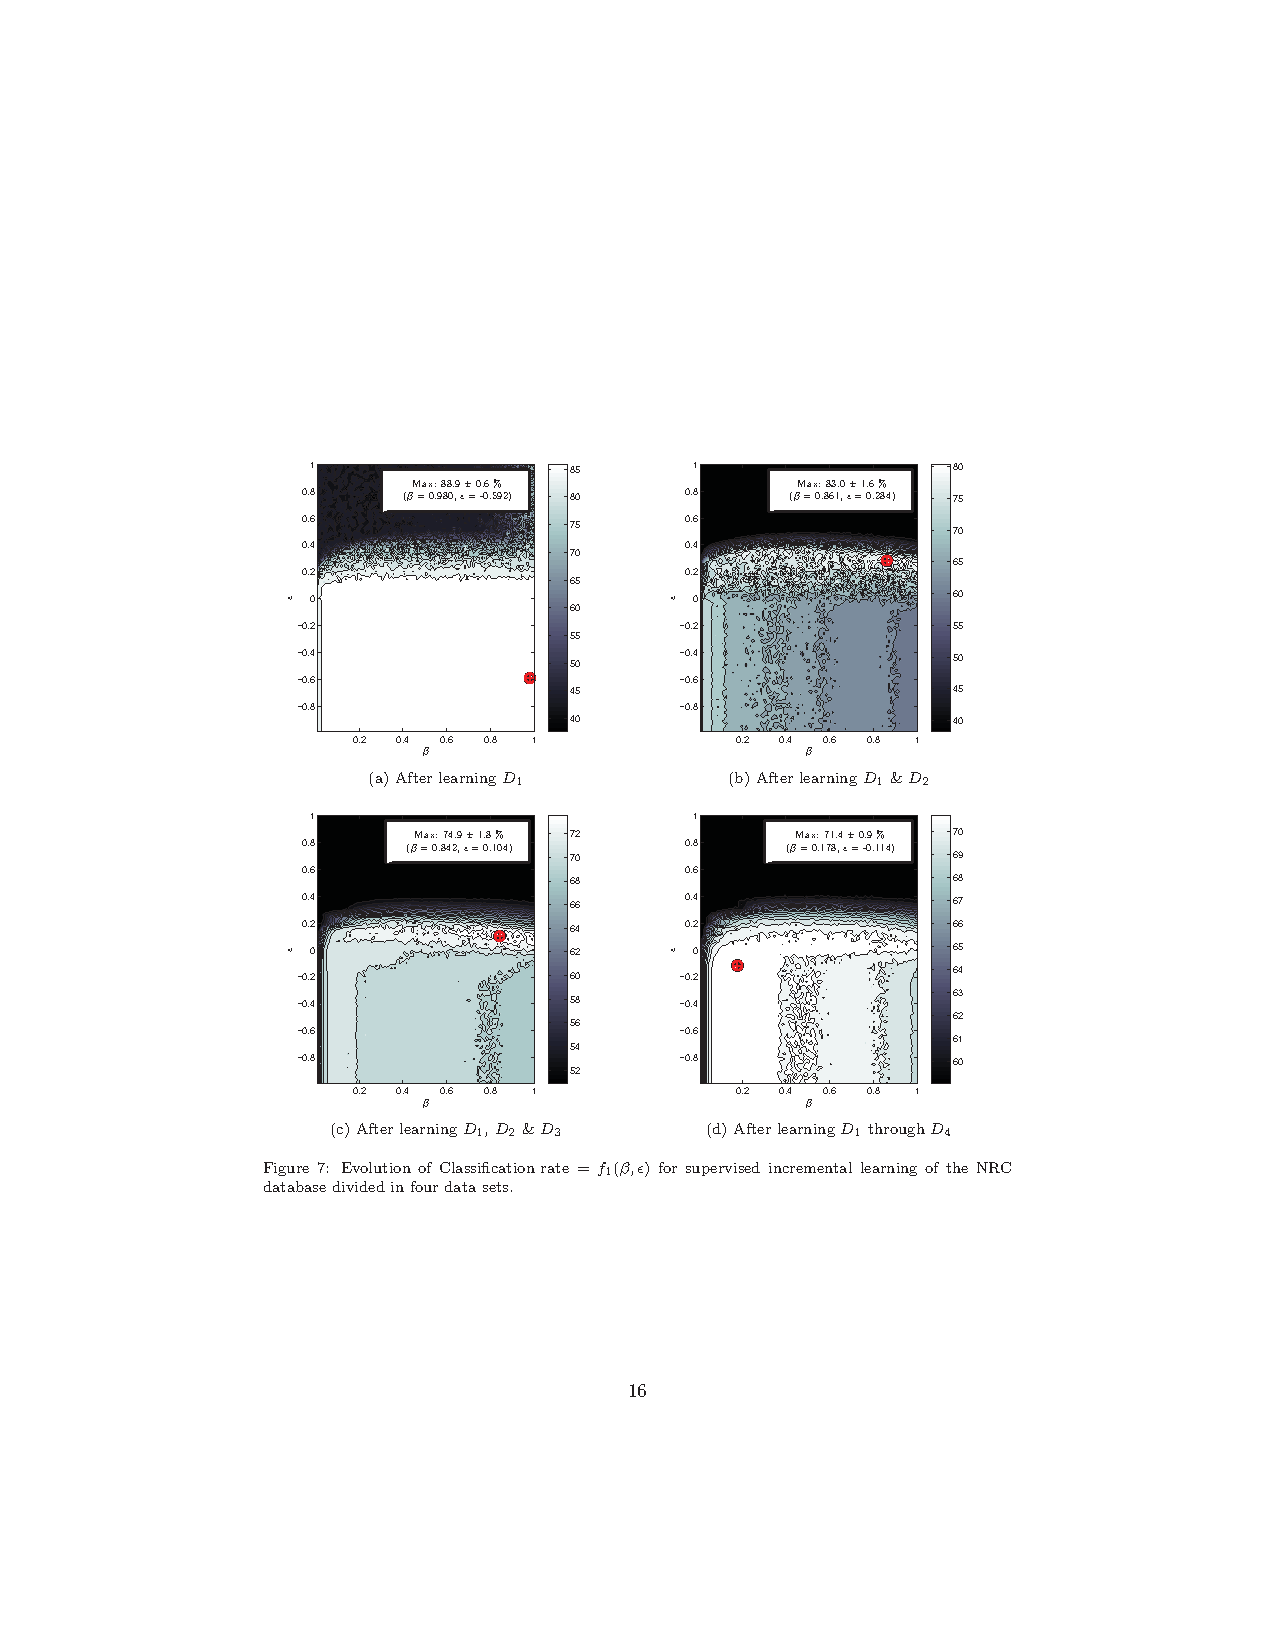
\includegraphics[width=0.45\linewidth, viewport= 4.8cm  15.1cm  9.9cm 20.2cm,
  								 clip] {c1_fig13} \label{fig:2d_1} &
  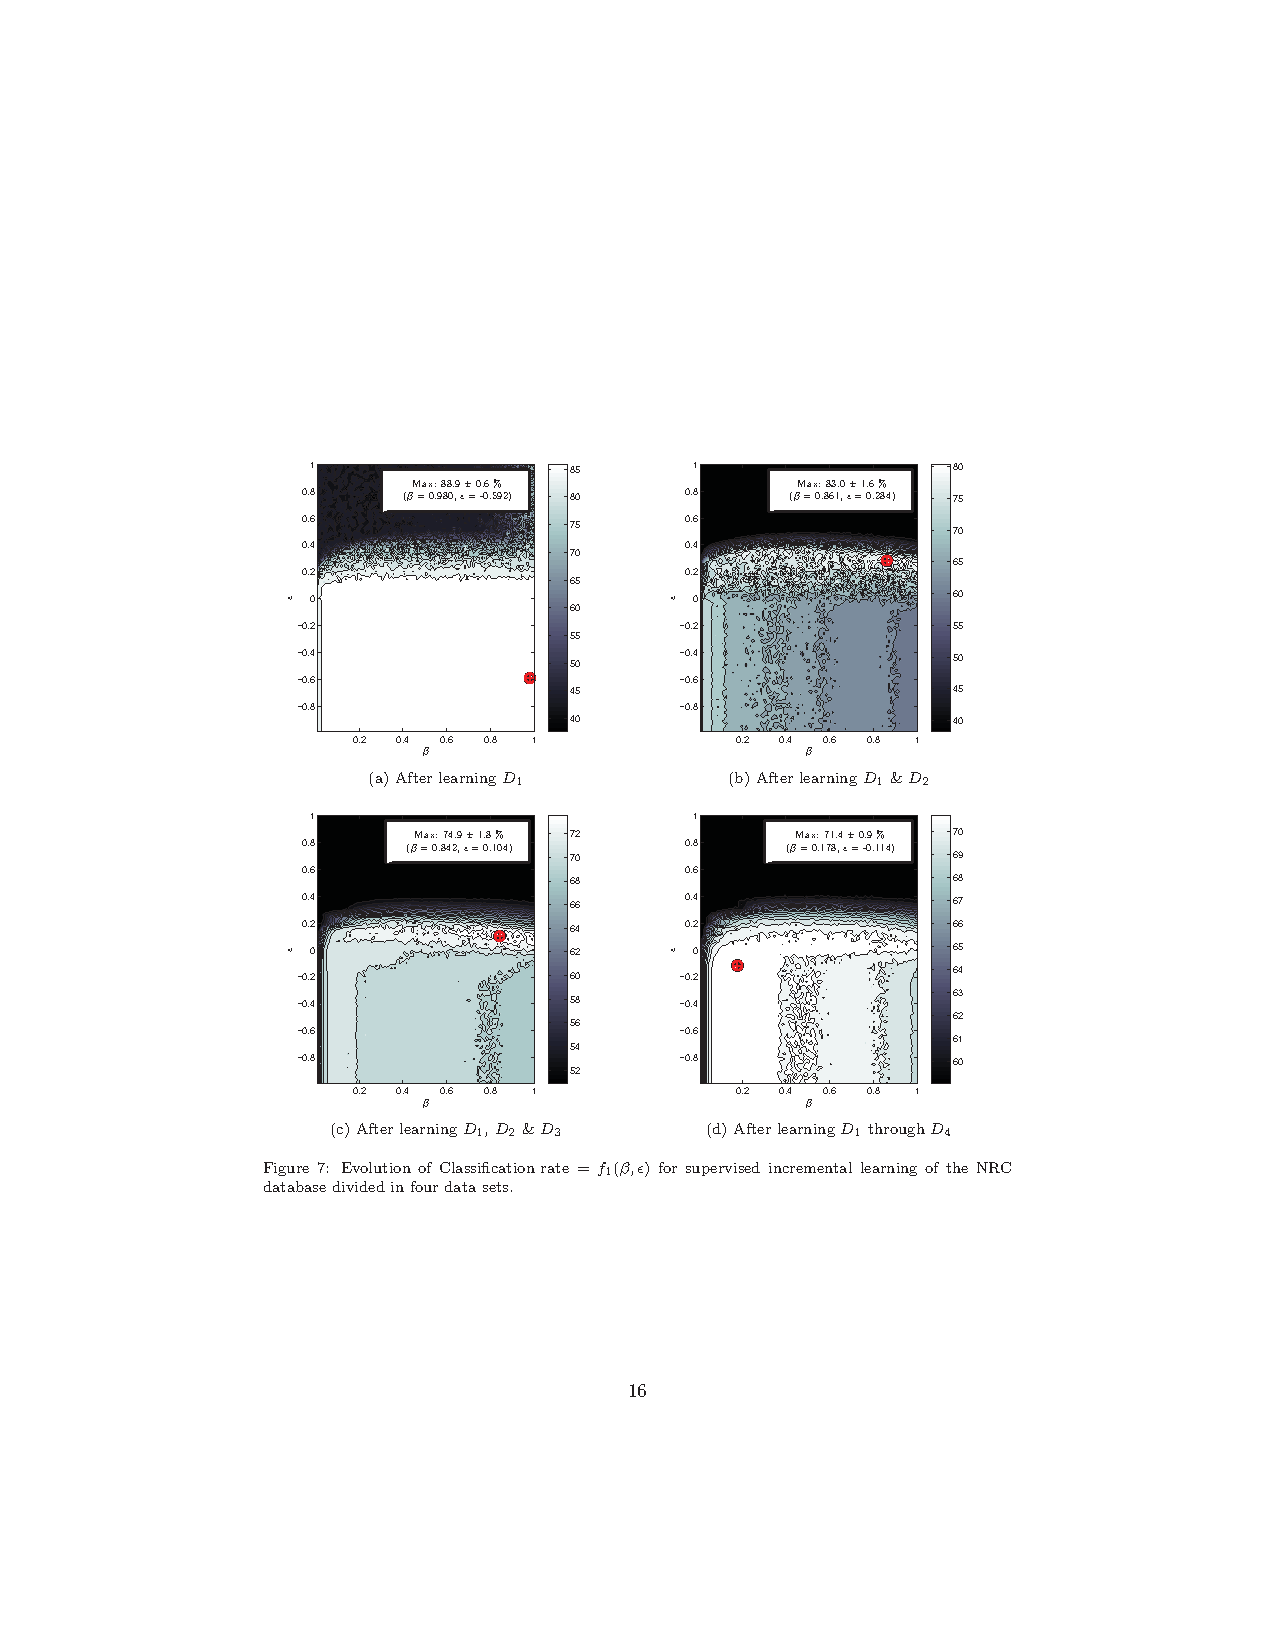
\includegraphics[width=0.45\linewidth, viewport= 11.3cm 15.1cm 16.3cm 20.2cm,
  								 clip] {c1_fig13} \label{fig:2d_2} \\
	\footnotesize{\textbf{(a)} $D_1$} & \footnotesize{\textbf{(b)} $D_2$}\\

  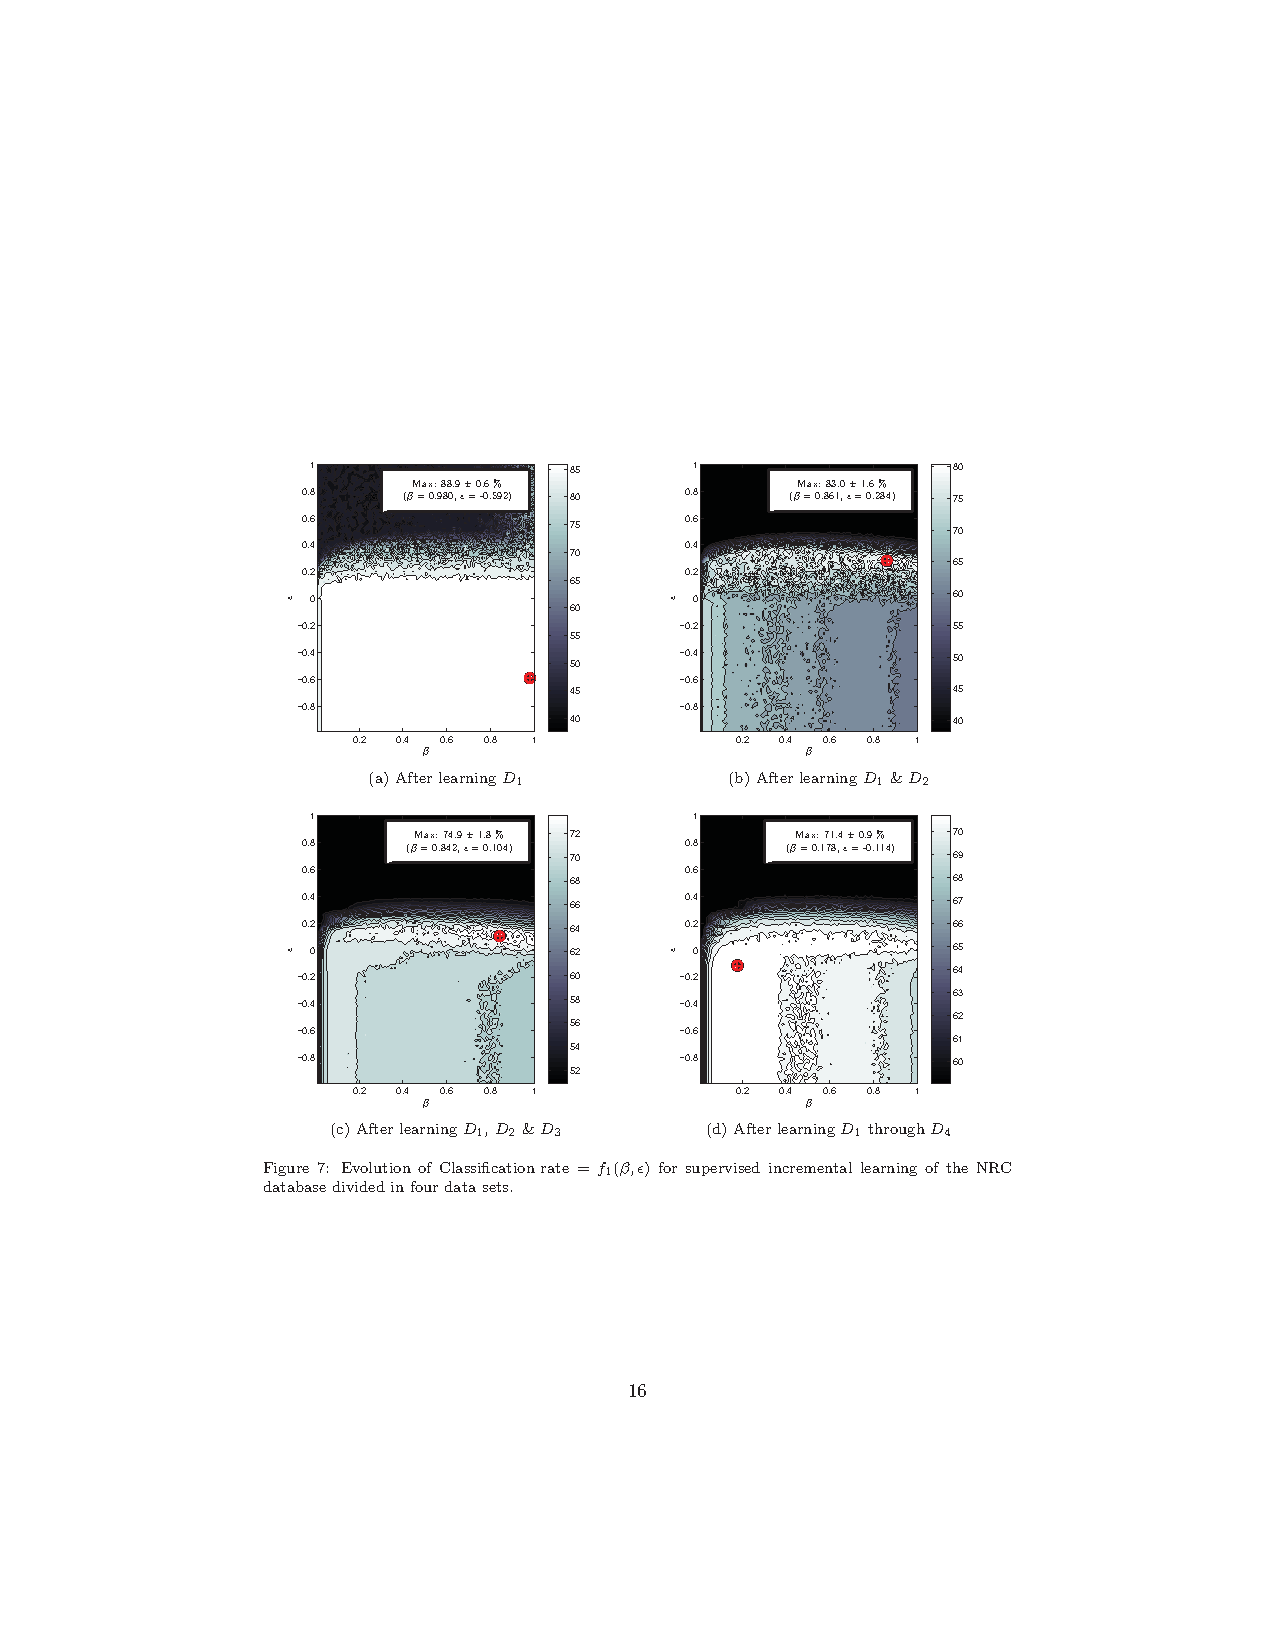
\includegraphics[width=0.45\linewidth, viewport= 4.8cm   9.2cm  9.9cm 14.4cm, 									 clip] {c1_fig13} &
  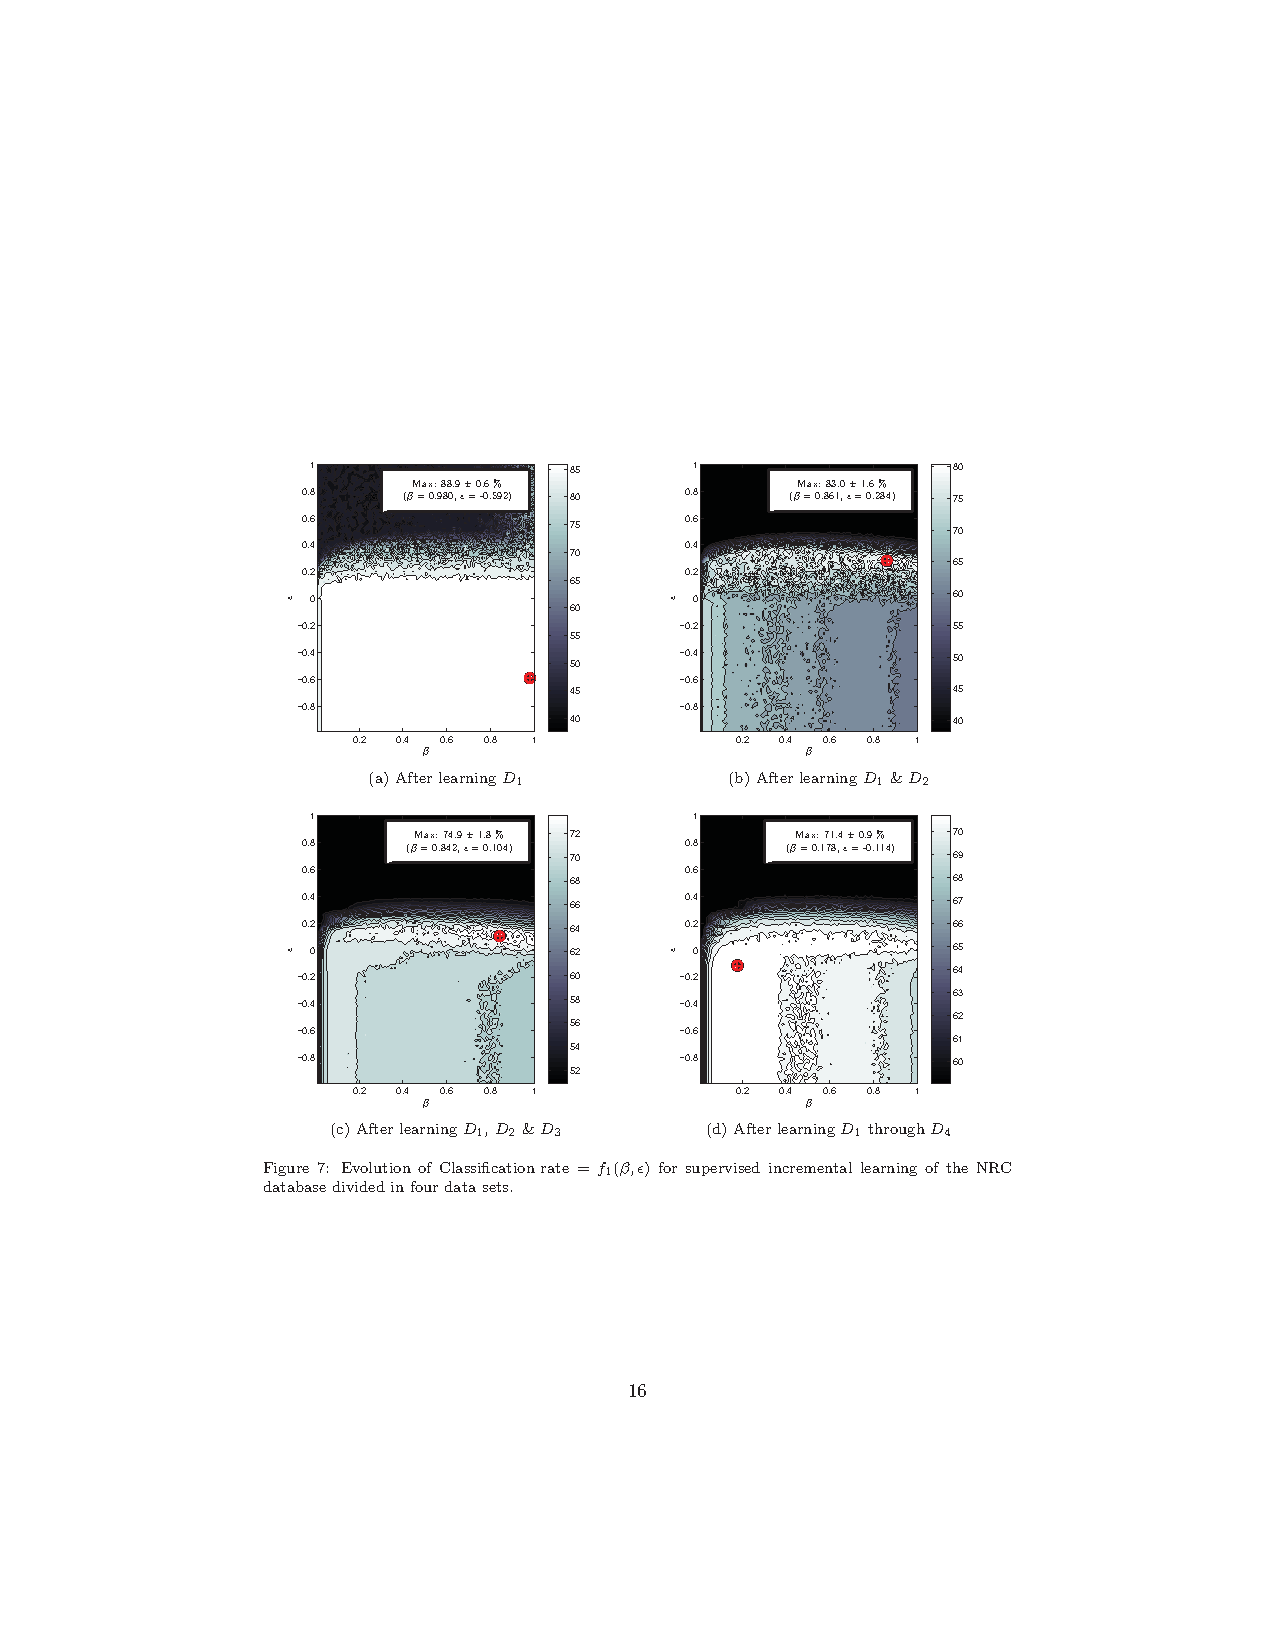
\includegraphics[width=0.45\linewidth, viewport= 11.3cm  9.2cm 16.3cm 14.4cm, 									 clip] {c1_fig13} \\
	\footnotesize{\textbf{(a)} $D_3$} & \footnotesize{\textbf{(b)} $D_4$}


	\end{tabular}	
	}
  \captionsetup{list=no}
	\caption{Evolution of the objective function $f(\textbf{h},t)$, where $\textbf{h}=(\beta, \epsilon)$, during an enrollment learning scenario of four learning data blocks $D_t$. The global maximum is shown along with its classification rate and its 90\% confidence interval}
	\label{fig:2Dresult}
\end{figure}
